\phantomsection

\chapter{Resultados}

Este capítulo apresenta os sinais e valores obtidos no experimento realizado no dispositivo de flexão. Os tópicos aqui analisados apresentam a comparação dos resultados
obtidos pelo experimento realizado pelo autor com os valores obtidos pelo estudo de caso feito por \autocite{Minela2017}.

O objetivo primário da comparação dos resultados é o de se obter dados descritivos de performance do dispositivo desenvolvido em relação a um sistema de medição industrial
homologado, no final do capítulo são indicados as situações de melhor performance do protótipo.

\section{Sinais obtidos}

Os sinais captados pelo sistema de medição desenvolvido seguem um formato trapezoidal, onde as zonas iniciais e finais representam os momentos em que a viga não se encontrava
sob a aplicação da carga, e a zona intermediária representa a total aplicação da carga no dispositivo.

\subsection{Sinais de calibração}

Nota-se que os valores obtidos sem cargas aplicadas não se igualam a valores nulos, isso acontece pois existe um diferencial de tensão entre os pólos da ponte de Wheatstone,
esse diferencial pode ser causado por imprecisão nos valores de resistência dos resistores utilizados, fatores térmicos na execução do experimento que alteram a resistência
do extensômetro, ou imprecisões ou ruídos que podem estar presentes nos componentes eletrônicos do amplificador de sinal utilizado.

\begin{figure}[htb]
	\caption{\label{fig:410} Sinal obtido sem a aplicação de cargas no dispositivo}
	\begin{center}
		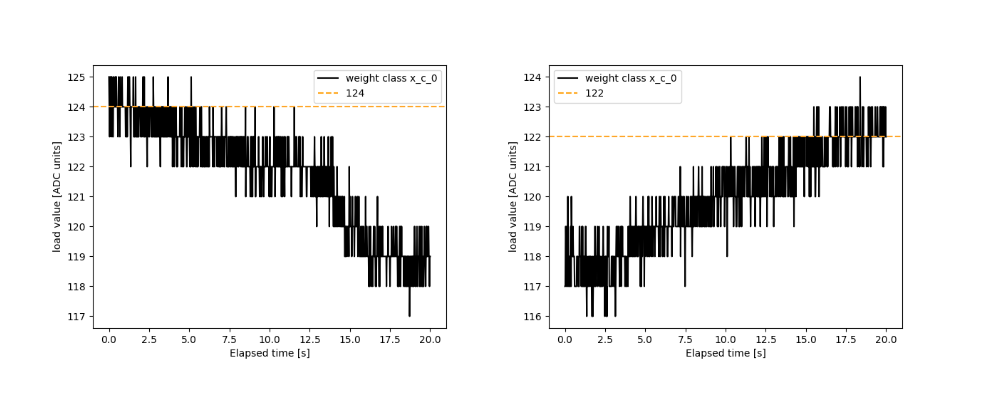
\includegraphics[width=\textwidth]{pictures/x_cal_0.png}
	\end{center}
	\fonte{O autor 2022}
\end{figure}

Uma vez que o sinal sem cargas aplicadas apresenta ruídos e flçutuações indesejadas, foi decidido a utilização de duas cargas para calibração do dispositivo, os sinais
obtidos pela aplicação das cargas são mostradas nas \autoref{fig:420} e \autoref{fig:430}
\begin{figure}[htb]
	\caption{\label{fig:420} Sinal obtido pela aplicação da cargas de calibração baixa}
	\begin{center}
		\includegraphics[width=\textwidth]{pictures/x_cal_1.png}
	\end{center}
	\fonte{O autor 2022}
\end{figure}

\begin{figure}[htb]
	\caption{\label{fig:430} Sinal obtido pela aplicação da cargas de calibração alta}
	\begin{center}
		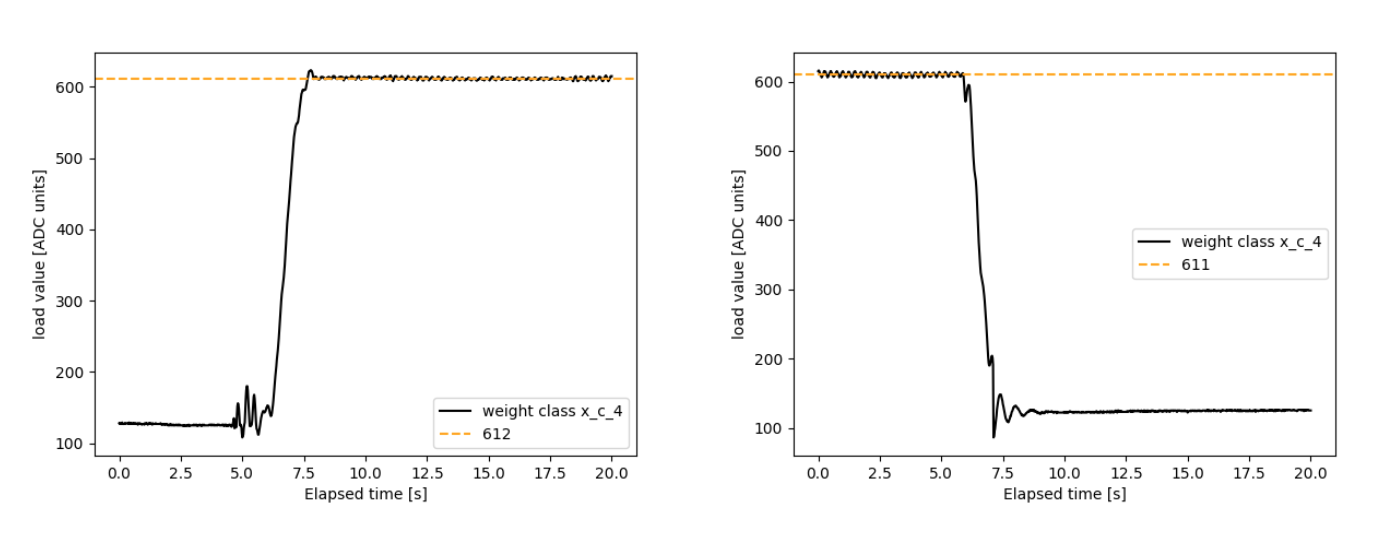
\includegraphics[width=\textwidth]{pictures/x_cal_4.png}
	\end{center}
	\fonte{O autor 2022}}
\end{figure}

%Após a calibração utilizando diferentes grandezas físicas como base são obtidos os dados demonstrados na \autoref{fig:4010}.

%\begin{figure}[htb]
%	\caption{\label{fig:440} Valores esperados conforme aplicação da carga na viga}
%	\begin{center}
%		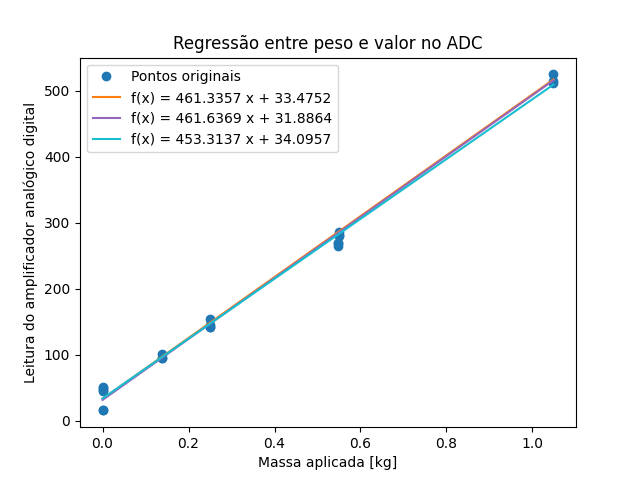
\includegraphics[width=\textwidth]{pictures/sep_24_1_weight.png}
%	\end{center}
%	\fonte{O autor 2022}}
%\end{figure}

\subsection{Ruídos presentes}


Os ruídos presentes no sinal se mostram de maior criticidade nas situações em que menores cargas são aplicadas.

\subsection{Valores nominais}

A \autoref{fig:4010} mostra os valores nominais de deformação para cada leitura da zona intermediária de cada sinal para cada combinação de cargas
realizadas na execução do experimento, assim como o valor médio das amostras para cada combinação e o desvio padrão dos dados na zona intermediária
de cada sinal como avaliação dos ruídos presentes.

\begin{figure}[htb]
	\caption{\label{fig:4010} Amostras e valores médios obtidos}
	\begin{center}
		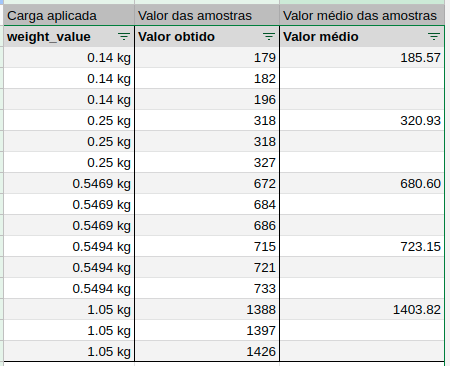
\includegraphics[width=\textwidth]{pictures/val_func_cal.png}
	\end{center}
	\fonte{O autor 2022}}
\end{figure}

%Os Valores de carga compensados pelo problema da porca e do peso não encontrados conforme indicado na \autoref{}, junto com a comparação dos resultados obtidos por
%\autocite{Minela2017} são mostrados na \autoref{}.

\section{Funções de ajuste}

A resolução das funções de minimização de mínimos quadrados é feita utilizando a função stats.linregress do pacote SciPy, foram analisados a influência da utilização
de quantidade e diferentes pontos nos indicadores obtidos na criação da função de ajuste, conforme a \autoref{fig:450}.

\begin{figure}[htb]
	\caption{\label{fig:450} Função de ajuste de dados de deformação em relação aos valores obtidos no amplificador}
	\begin{center}
		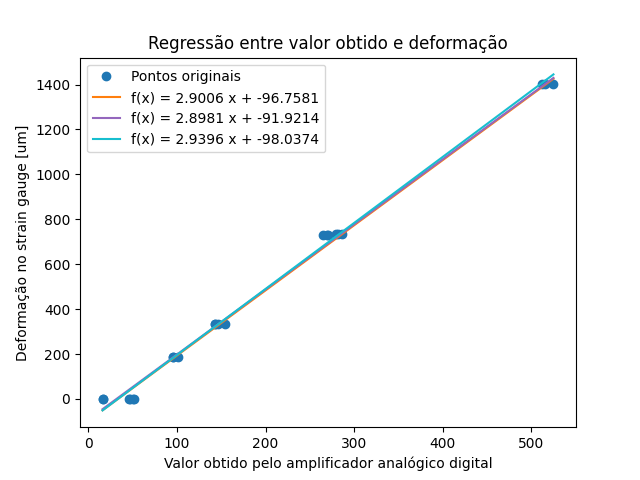
\includegraphics[width=\textwidth]{pictures/sep_24_1_deformation.png}
	\end{center}
	\fonte{O autor 2022}}
\end{figure}

\begin{figure}[htb]
	\caption{\label{fig:4020} Comparação dos valores convertidos usando diferentes funções de ajuste}
	\begin{center}
		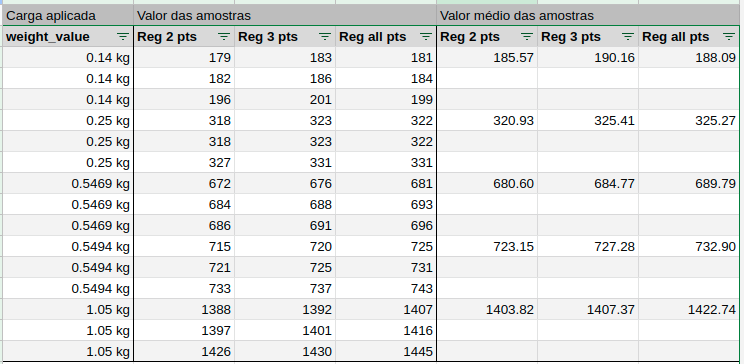
\includegraphics[width=\textwidth]{pictures/comp_func_reg.png}
	\end{center}
	\fonte{O autor 2022}}
\end{figure}

\begin{figure}[htb]
	\caption{\label{fig:4020} Erro entre valores encontrados com a função de ajuste e os valores esperados pela análise analítica}
	\begin{center}
		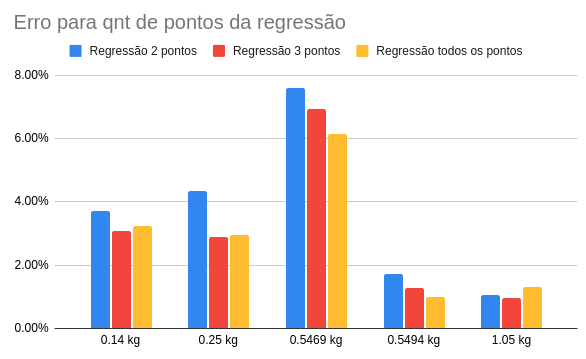
\includegraphics[width=\textwidth]{pictures/comp_func_reg_erros.png}
	\end{center}
	\fonte{O autor 2022}}
\end{figure}

%\section{Comparação final}
%
%A \autoref{} compara os principais resultados obtidos pelo experimento desenvolvido pelo autor com os resultados obtidos pelo trabalho de \autocite{Minela2017}.
